% !TeX program = lualatex
% !BIB program = biber
% Lualatex is important to render TTF fonts; with pdflatex it's just the regular one
% ratio 16:9 -- https://tex.stackexchange.com/questions/14336/

% compile two versions, inspired by https://tex.stackexchange.com/a/1501
% use the script "compile-pdf.sh"
\newif\ifhandout
% if flags.tex does not exist, create an empty file to be able to compile in TeXstudio
\input{flags}

\ifhandout
\documentclass[12pt,aspectratio=169,handout]{beamer}
\else
\documentclass[12pt,aspectratio=169]{beamer}
\fi



% TODO change "leftfootertext" to your liking
\newcommand{\leftfootertext}{\insertsubtitle}  % just the \title{} text by default
%\newcommand{\leftfootertext}{AI is all you need | Dr.\ Maria Mustermann}  % Your name, for instance


% ------- RUB specifics ----------
% adjust for 16:9
% https://tex.stackexchange.com/questions/354022/modifying-the-margins-of-all-slides-in-beamer
\setbeamersize{text margin left=0.3cm,text margin right=4.5cm} 


% use Metropolis as the basis theme
\usetheme[subsectionpage=progressbar]{metropolis}
% blocks with background globally
\metroset{block=fill}


\usepackage{fontspec}
% RUB fonts need to be installed
% 'UprightFont = * Light' makes sure that the base font is RubFlama Light, which looks
% lighter than RubFlama Regular (would be too thick for slides)
\setsansfont[Scale=MatchLowercase, UprightFont = * Light, BoldFont = * Bold]{RubFlama}
%\setsansfont{Arial} % Open source alternative if you don't have RubFlama

% RUB color scheme
% Dark blue: 0; 53; 96; #003560
\definecolor{RUBDarkBlue}{RGB}{0, 53, 96}

% Light yellow (table fill, etc.); 238; 250; 196; #EEFAC4
\definecolor{RUBLightYellow}{RGB}{238, 250, 196}

%Light green: 141; 174; 16
\definecolor{RUBLightGreen}{RGB}{141, 174, 16}


\setbeamercolor{titlelike}{fg=RUBDarkBlue}
\setbeamercolor{subtitle}{fg=RUBLightGreen}
\setbeamercolor{separation line}{fg=RUBLightGreen}
\setbeamercolor{frametitle}{bg=white, fg=RUBDarkBlue}

% horizontal line on title page and sections
\setbeamercolor{alerted text}{fg=RUBLightGreen}


% Adjust footer bottom (too large by default)
\setbeamertemplate{footline}{%
  \begin{beamercolorbox}[wd=\textwidth, sep=2ex]{footline}%
    \usebeamerfont{page number in head/foot}%
    \usebeamertemplate*{frame footer}
    \hfill%
    \usebeamertemplate*{frame numbering}
  \end{beamercolorbox}%
}


% Lab name, numbering, etc. in footer
\setbeamertemplate{frame numbering}{TrustHLT --- Prof.\ Dr.\ Ivan Habernal \hspace*{1ex} 
\includegraphics[width=7em]{img/rub-logo.pdf}\hspace*{1ex}}

\setbeamertemplate{frame footer}{\hspace*{1ex}\insertframenumber \hspace*{2ex} \leftfootertext}

% adjust the background to be completely white
\setbeamercolor{background canvas}{bg=white}

% logos on the title page
\titlegraphic{%
	\begin{picture}(0,0)
		\put(435,0){\makebox(0,0)[rt]{
\includegraphics[width=7em]{img/rub-logo.pdf}}}
		\put(435,-170){\makebox(0,0)[rt]{
\includegraphics[width=4em]{img/logo-trusthlt.pdf}}}
		\put(435,-196){\makebox(0,0)[rt]{
\includegraphics[width=9em]{img/logo-rctrust.pdf}}}
	\end{picture}%
}


% show TOC at every section start
\AtBeginSection{
	\frame{
		\vspace{2em}
		\sectionpage
		\hspace*{2.2em}\begin{minipage}{10cm}
			\tableofcontents[currentsection]
		\end{minipage}
	}
}

% TOC without subsection
\setcounter{tocdepth}{1} % only-- part,chapters,sections 

% bullet points: rectangles
\useinnertheme{rectangles}
\setbeamercolor{itemize item}{fg=RUBLightGreen}
\setbeamercolor{itemize subitem}{fg=RUBLightGreen}
% enumerate: blue background for better readability
\setbeamercolor{item projected}{bg=RUBDarkBlue}

% make boxes (example, block, etc.) background lighter for readability
\setbeamercolor{block title}{%
	use=normal text,
	fg=normal text.fg,
	bg=normal text.bg!90!fg % lighter background in block title
}
\setbeamercolor{block body}{
	use={block title, normal text},
	bg=block title.bg!30!normal text.bg % lighter background in block body
}


% RUB colors in blocks
\setbeamercolor{block title alerted}{%
	use={block title, alerted text},
	bg=RUBDarkBlue,
	%fg=RUBLightYellow % looks bad
	fg=white % better contrast
}

\setbeamercolor{block title example}{%
	use={block title, example text},
	fg=RUBLightGreen
}


% ------- end of RUB specifics ----------

% all itemize with pause by default
%\beamerdefaultoverlayspecification{<+->}


% typeset mathematics on serif
\usefonttheme[onlymath]{serif}

% better bibliography using biber as backend
\usepackage[natbib=true,backend=biber,style=authoryear-icomp,maxbibnames=30,maxcitenames=9,uniquelist=false,giveninits=true,doi=false,url=false,dashed=false,isbn=false]{biblatex}
% shared bibliography
\addbibresource{../../nlpwdl-bibliography.bib}
% disable "ibid" for repeated citations
\boolfalse{citetracker}



\usepackage{xspace}


% for derivatives, https://tex.stackexchange.com/a/412442
\usepackage{physics}

\usepackage{tikz}
\usetikzlibrary{matrix, positioning}
\usetikzlibrary{angles,quotes} % for angles
\usetikzlibrary{backgrounds} % background
\usetikzlibrary{decorations.pathreplacing} % curly braces
\usetikzlibrary{calligraphy}
\usetikzlibrary{calc} % for neural nets

% for plotting functions
\usepackage{pgfplots}
\usepgfplotslibrary{dateplot}

% sub-figures
\usepackage{caption}
\usepackage{subcaption}

% book tabs
\usepackage{booktabs}


% argmin, argmax
\usepackage{amsmath}
\DeclareMathOperator*{\argmax}{arg\!\max}
\DeclareMathOperator*{\argmin}{arg\!\min}
% softmax
\DeclareMathOperator*{\softmax}{soft\!\max}
% Mask
\DeclareMathOperator*{\mask}{mask}

% bold math
\usepackage{bm}

% for \mathclap
\usepackage{mathtools}

% algorithms
\usepackage[noend]{algpseudocode}


% for neurons and layers in tikz
\tikzset{
	neuron/.style={draw, rectangle, inner sep=2pt, minimum width=0.75cm, fill=blue!20},
	param/.style={draw, rectangle, inner sep=2pt, minimum width=0.75cm, fill=green!20},
	constant/.style={draw, rectangle, inner sep=2pt, minimum width=0.75cm, fill=black!15},
	% for citation nodes right top
	ref/.style={anchor = north east, text width=7.8cm, yshift=-1.3cm, xshift=-0.2cm, scale=0.5},
	state/.style={rectangle, inner sep=2pt, minimum width=0.75cm, fill=black!5},
}

% added in lecture 10
\tikzset{
	mtx/.style={
		matrix of math nodes,
		left delimiter={[}, right delimiter={]}
	},
	hlt/.style={opacity=0.1, line width=4 mm, line cap=round},
	hltr/.style={opacity=0.5, rounded corners=2pt, inner sep=-1pt}
}

% for strike-through text (added in Lecture 06)
\usepackage[normalem]{ulem}

% added in Lecture 7
% RNN
\DeclareMathOperator*{\rnn}{RNN}
% RNN star
\DeclareMathOperator*{\rnnstar}{RNN^{*}}
% bi-RNN
\DeclareMathOperator*{\birnn}{biRNN}


% added in Lecture 9
\usetikzlibrary{fit} % for hightligting by calling "fit"

% algorithms
\usepackage[noend]{algpseudocode}



\title{Natural Language Processing with Deep Learning}
\subtitle{Lecture 3 --- Mathematical foundations of deep learning}
\date{October 31, 2024}
\author{Prof.\ Dr.\ Ivan Habernal}
\institute{
\texttt{www.trusthlt.org} \\
Trustworthy Human Language Technologies Group (TrustHLT) \\
Ruhr University Bochum \& Research Center Trustworthy Data Science and Security}


\begin{document}

\maketitle



\section{Motivation}

\begin{frame}{Why finding a minimum of a function matters?}
	
In supervised machine learning ...
	
\pause

	\begin{itemize}
		\item We have some training data (e.g., for classification)
		\item We have a learning algorithm
		\item We want to minimize some kind of error (e.g., misclassification) of the learning algorithm on training data
	\end{itemize}

\end{frame}


%\begin{frame}{How deep will we go?}
%	We won't cover
%	
%	\begin{itemize}
%		\item Set theory: The assembler of mathematics
%		\begin{itemize}
%			\item Sets $A = \{a, b, c\}$, $a \in A$, no ordering
%			\item Ordered tuples $(a, b) \neq (b, a)$
%		\end{itemize}
%		\pause
%		\item Number theory
%		\begin{itemize}
%			\item Set of natural numbers $\mathbb{N}_0 = \{0, 1, \ldots\}$
%			\item Set of real numbers $\mathbb{R}$, infinity
%		\end{itemize}
%		\pause
%		\item Sequences and limits
%	\end{itemize}
%	
%	$\mathbb{R}^2 = \mathbb{R} \times \mathbb{R}$ --- tuples of reals, e.g., $(1.3, -44.67)$, also a two-dimensional vector
%	
%	
%\end{frame}


\section{Problem 1: Minimize functions}




\begin{frame}{Problem: Find minimum of any function}
	
	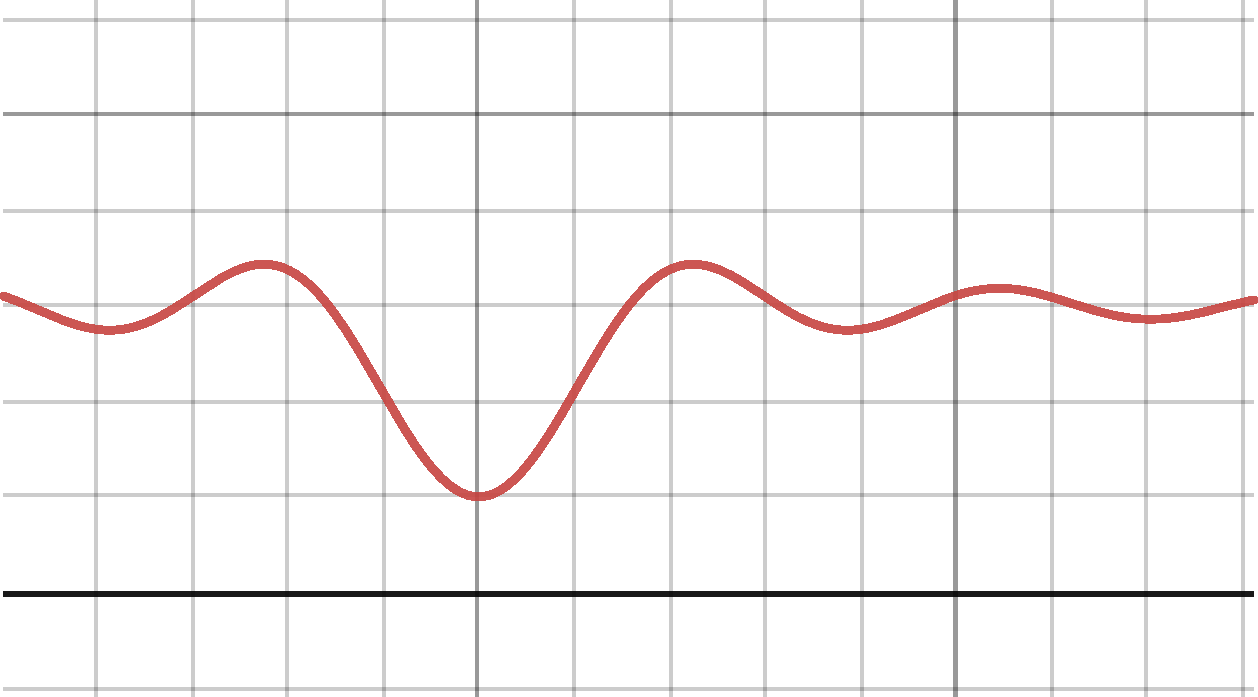
\includegraphics[width=0.7\linewidth]{img/desmos-graph1.pdf}
	
	\begin{itemize}
		\item For "easy" functions, closed-form solution (high school math)
		\item For complicated functions not trivial and cumbersome
	\end{itemize}
	
	
	
\end{frame}







\begin{frame}{Function of single variable}
	
	We typically use Euler's notation with arbitrary but somehow standard naming conventions ($x, y, f$)
	
	$y = f (x) \qquad f: \mathbb{R} \to \mathbb{R}$
	
	$f : A \to B$ where $A$ is domain, $B$ is co-domain
	
	\bigskip
	
	\begin{block}{Function composition}
		$f: \mathbb{R} \to \mathbb{R} \quad g: \mathbb{R} \to \mathbb{R}$
		
		$h = g \circ f$
		
		$h(x) = g(f(x))$ or $(g \circ f)(x)= g(f(x))$
	\end{block}
	
\end{frame}


\begin{frame}{Lines in two dimensions}
	
	Lines in a Cartesian plane are characterized by linear equations.
	
	Every line $L$ (including vertical lines) is the set of all points whose coordinates $(x, y)$ satisfy a linear equation:
	
	$L=\{(x,y)\mid w_1 x+ w_2 y= w_3\}$
	
	where $w_1$, $w_2$ and $w_3$ are fixed real numbers (called coefficients) such that $w_1$ and $w_2$ are not both zero.
	
\end{frame}


\begin{frame}{Linear function in two dimensions}
	
	Usually we use \textbf{slope-intercept} form $y= a x + b$
	
	
	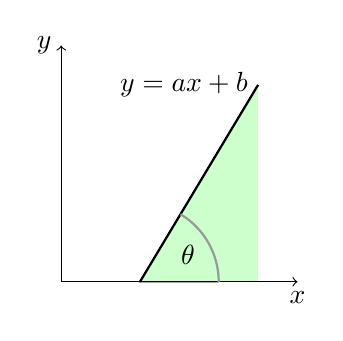
\begin{tikzpicture}
		
		\draw[->] (0,0)--(3,0) node[below]{$x$};
		\draw[->] (0,0)--(0,3) node[left]{$y$};
		\draw[-, thick] (1,0)--(2.5,2.5) node[left]{$y = ax + b$};
		
		
		\draw
		(2,1.666) coordinate (a)
		-- (1,0) coordinate (b)
		-- (2,0) coordinate (c)
		pic["$\theta$", draw=black!40, thick, -, angle eccentricity=0.7, angle radius=1cm]
		{angle=c--b--a};
		
		\begin{scope}[on background layer]
			\path [fill=green!20] (1,0) -- (2.5,2.5) -- (2.5,0) -- cycle;
		\end{scope}
		
	\end{tikzpicture}
	
	$\theta = \arctan (a) \qquad a = \tan (\theta)$
	
\end{frame}



\begin{frame}{Approximate function by a line at point}
	
	%\includegraphics[width=0.5\linewidth]{img/f2.png}
	
	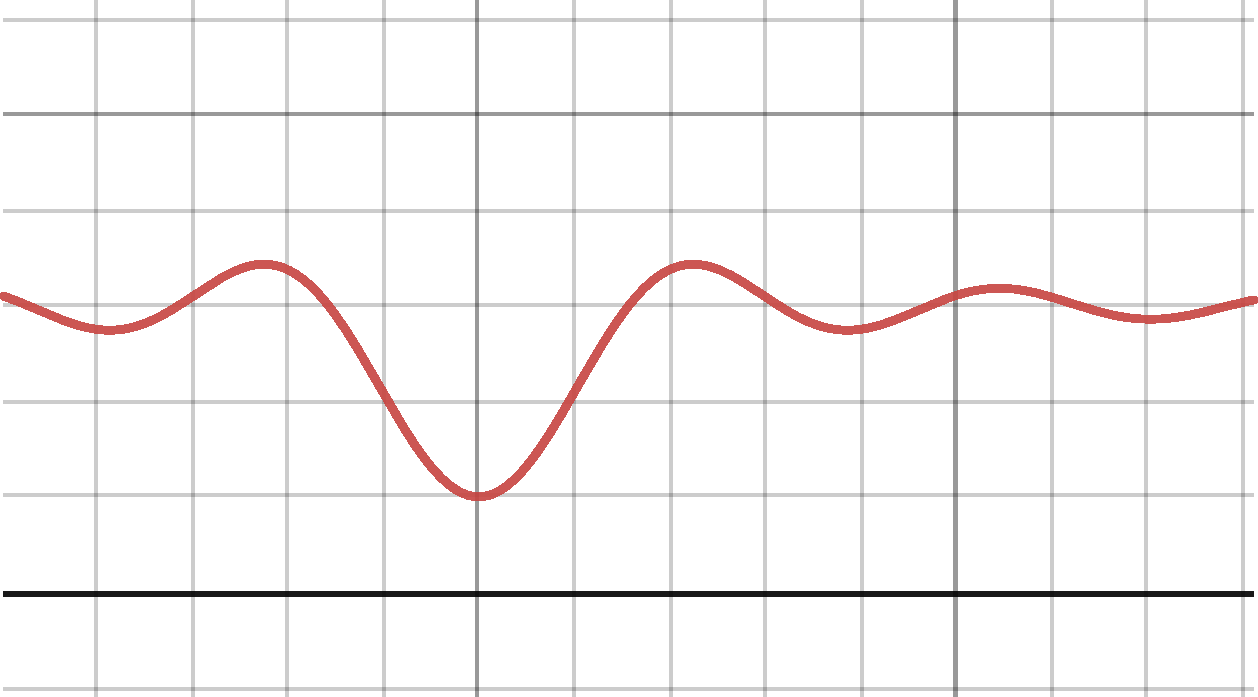
\includegraphics[width=0.7\linewidth]{img/desmos-graph1.pdf}
	
	
	%3-\frac{\sin\left(2x\right)}{x}
	
	
	"Steepness" at $c$?
	$$f'(c) = \lim_{x \to c} \frac{f(x) - f(c)}{x - c}$$
	The derivative of $f$ at $c$
	
	
	
	
	
\end{frame}


\begin{frame}{Derivative-computing function}
	
	We want a function $D$ which, when given a differentiable function $f : \mathbb{R} \to \mathbb{R}$ as input, produces another function $g : \mathbb{R} \to \mathbb{R}$ output, such that $g(c) = f'(c)$ for every $c$.
	
	\bigskip
	\pause
	This derivative-computing function $D$ is often written as 
	$$\frac{d}{dx}$$
	but this causes inconsistent notation like
	$$\frac{d}{dx}(f), \qquad \frac{df}{dx}, \qquad \frac{dy}{dx}$$
	and forces one to choose a variable name $x$ or $y$
	
\end{frame}

\begin{frame}{Derivative of nested functions: The chain rule hammer}
	
	%We "know" derivatives for trivial functions, e.g.
	%$f: y =  x^2 \qquad \frac{dy}{dx} = 2 x$
	
	\begin{block}{Variant 1 (Lagrange's notation)}
		Let $f, g : \mathbb{R} \to \mathbb{R}$ be two functions which have derivatives. Then the derivative of $g (f(x))$ is $g' (f(x)) \cdot f' (x)$
	\end{block}
	\pause
	
	\begin{block}{Variant 2 (Function composition operator $\circ$)}
		Let $f, g : \mathbb{R} \to \mathbb{R}$ be two functions which have derivatives. Let $h = g \circ f$. The derivative of $h$ is $h'=(g \circ f)'=(g'\circ f)\cdot f'$
	\end{block}
	\pause
	
\begin{block}{Variant 3 (Leibniz's notation)}
		Call $h(x) = g(f(x))$. Then using $\frac{dh}{dx}$ for the derivative of $h$, the chain rule for this would be $\frac{dh}{dx} = \frac{dh}{df} \frac{df}{dx}$
	\end{block}
	
\end{frame}


\begin{frame}{Chain rule example}
	
	Consider $y=e^{\sin(x^{2})}$. Composite of three functions:
	$$
	\begin{aligned}
		y &= f(u) = e^u \\
		u &= g(v) = \sin v = \sin (x^2) \\
		v &= h(x) = x^2
	\end{aligned}
	$$
	\pause
	Their derivatives are
	$$
	\begin{aligned}
		\frac{dy}{du} &= f'(u) = e^u = e^{\sin(x^{2})} \\
		\frac{du}{dv} &= g'(v) = \cos v = \cos (x^2) \\
		\frac{dv}{dx} &= h'(x) = 2x
	\end{aligned}
	$$
\end{frame}


\begin{frame}{Chain rule example (cont.)}
	
	Consider $y=e^{\sin(x^{2})}$. Composite of three functions:
	$$y = f(u) = e^u, u = g(v) = \sin v = \sin (x^2), v = h(x) = x^2$$
	Their derivatives are
	$$\frac{dy}{du} = e^{\sin(x^{2})}, \frac{du}{dv} = \cos (x^2), \frac{dv}{dx} = 2x$$
	
	\pause
	
	Derivative of their composite at the point $x = a$ is (in Leibniz notation)
	$$
	{\frac {dy}{dx}}=\left.{\frac {dy}{du}}\right|_{u=g(h(a))}\cdot \left.{\frac {du}{dv}}\right|_{v=h(a)}\cdot \left.{\frac {dv}{dx}}\right|_{x=a}
	$$
	
\end{frame}


\begin{frame}{Gradient-based optimization: Find minimum of a function}
	
	We want $\hat{x} = \argmin_x f(x)$
	
	Pre-requisites:
	
	\begin{itemize}
		\item We can evaluate $y = f(x)$ for any $x$
		\item We can evaluate its derivative $f'(c)$ (or $\frac{dy}{dx}(c)$) for any $c$
	\end{itemize}
	
	\begin{figure}
		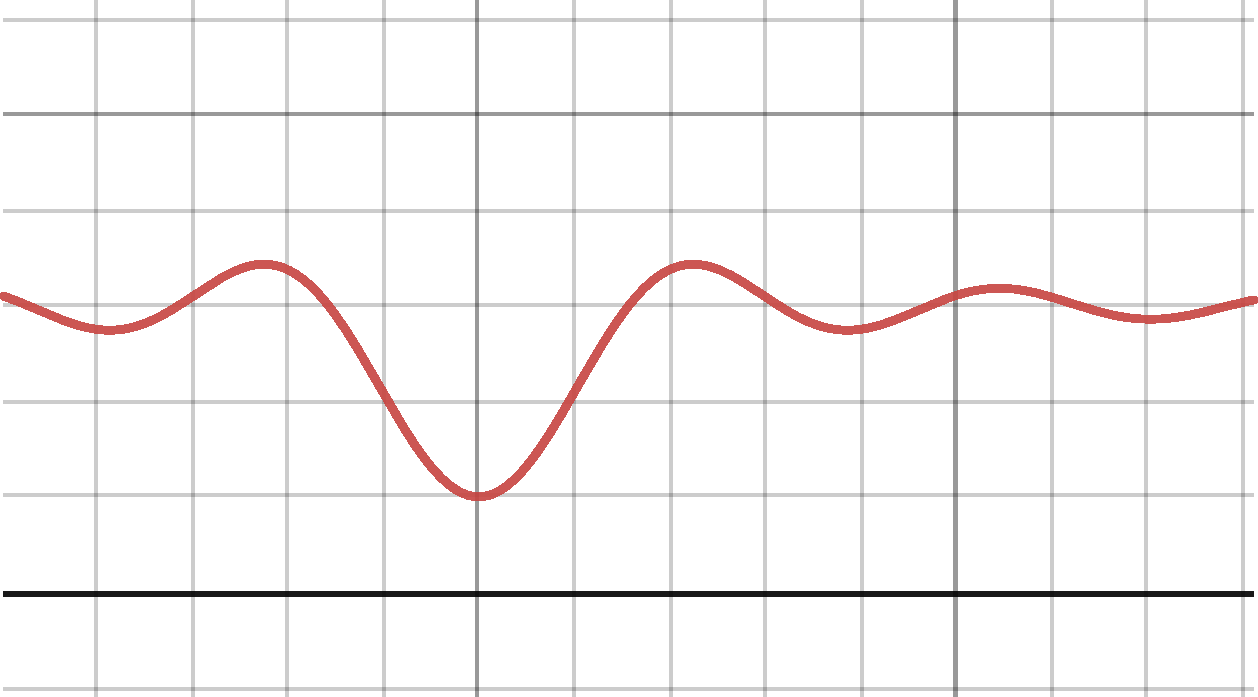
\includegraphics[width=0.4\linewidth]{img/desmos-graph1.pdf}	
		\caption{$3-\frac{\sin\left(2x\right)}{x}$}
	\end{figure}
	
\end{frame}


\begin{frame}{Gradient-based optimization: Find minimum of a function}
	
	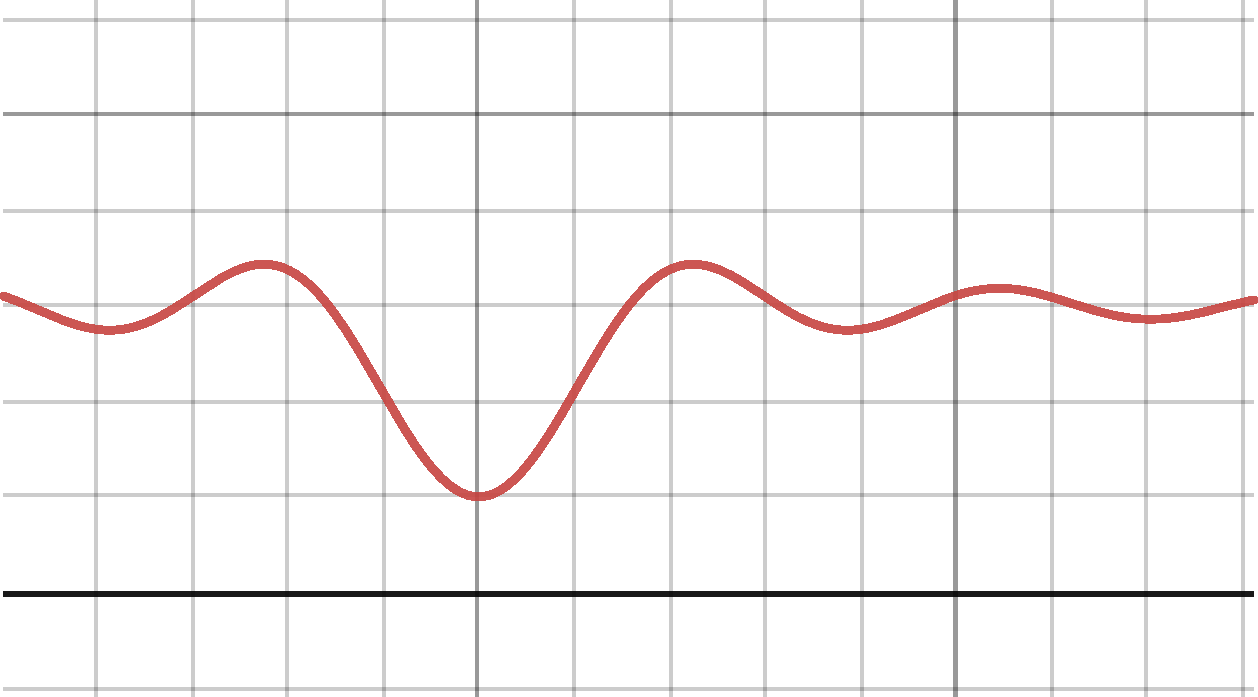
\includegraphics[width=0.4\linewidth]{img/desmos-graph1.pdf}
	
	
	\begin{enumerate}
		\item Start with initial random value $x_i$
		\item $u = f'(x_i)$ --- direction and strength of change at $x_i$
		\item Next value $x_{i + 1} \gets x_i - \eta \cdot u$
		\item With small enough $\eta$ (eta), $f(x_{i+1}) < f(x_i)$
	\end{enumerate}
	Repeating 2 + 3 (with properly decreasing values of $\eta$) will find minimum point $x_i$
	
	
	
\end{frame}


\begin{frame}{Gradient-based optimization: Workout example}
	
	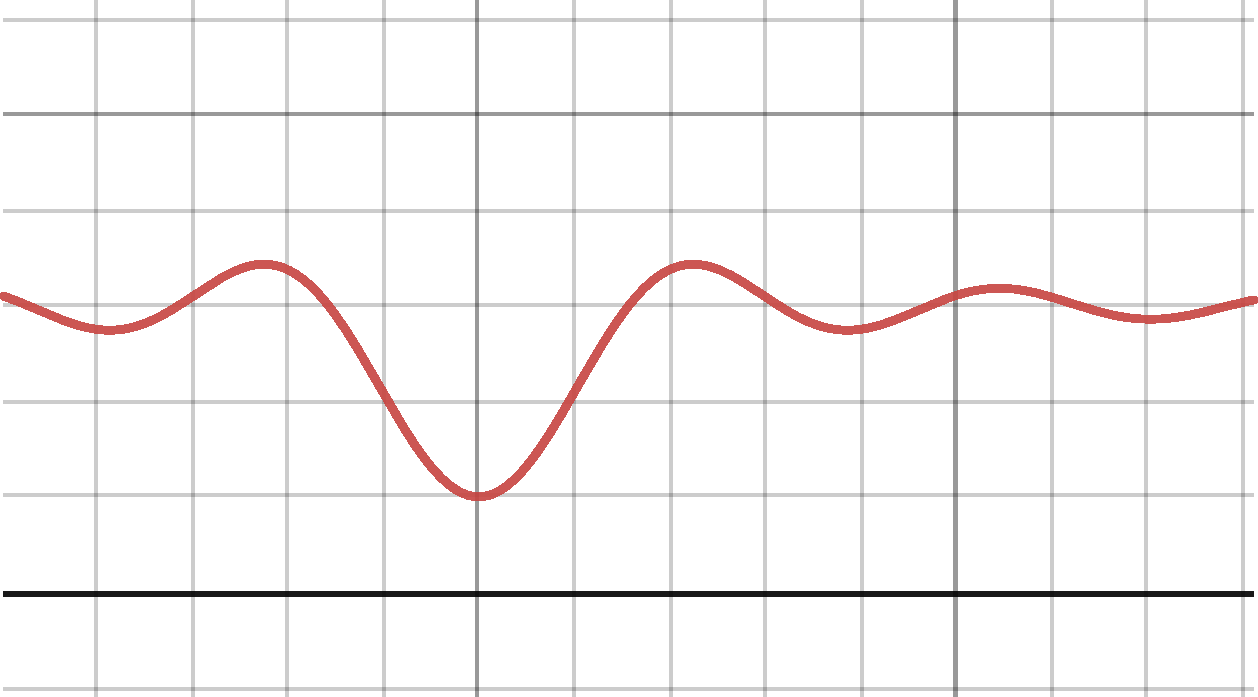
\includegraphics[width=0.99\linewidth]{img/desmos-graph1.pdf}
	
	
\end{frame}


\section{Problem 2: Minimize multivariate functions}

\begin{frame}{Multivariate functions $f: \mathbb{R}^n \to \mathbb{R}$}

	\begin{figure}
		\centering
		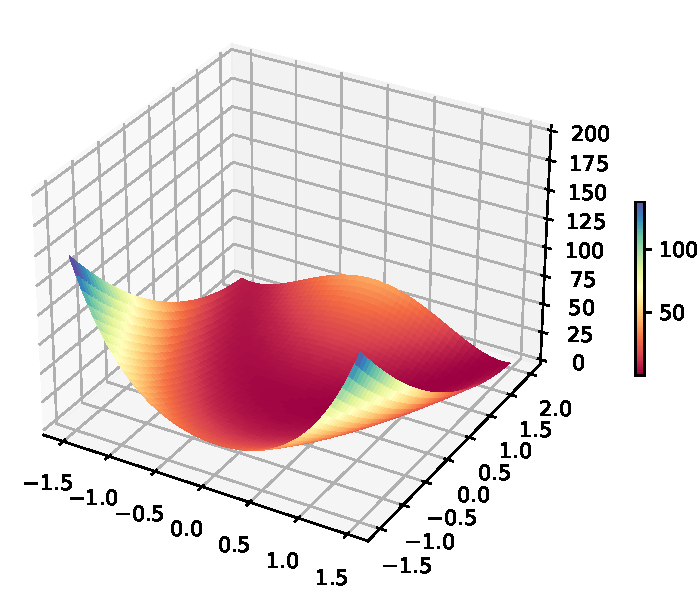
\includegraphics[trim={0 0.1cm 0 0.8cm},clip,width=0.55\linewidth]{img/rosenbrock.pdf}
		\caption{$f(x,y)=(a-x)^{2}+b(y-x^{2})^{2}, a = 1, b = 100$}
	\end{figure}
{\tiny \url{https://colab.research.google.com/drive/1mlZtxPXuk3mls56CQArmDzjdp5bLbrJC}}

\end{frame}




\begin{frame}{Partial derivatives}
	
	Partial derivative: the directional derivative wrt.\ a single variable
	
	\bigskip
	
	$\pdv{f}{x_2}$ --- "the partial derivative of $f$ with respect to $x_2$"
	
	\bigskip
	
	\begin{block}{Example: $f(x_1, x_2, x_3) = (x_1)^2 x_2 + \cos(x_3)$}
		$$
		\pdv{f}{x_1} = 2 x_2 x_1 \qquad \pdv{f}{x_2} = (x_1)^2 \qquad \pdv{f}{x_3} = - \sin (x_3)
		$$
	\end{block}
	
	
\end{frame}


\begin{frame}{Gradient}
	
	\begin{block}{Example: $f(x_1, x_2, x_3) = (x_1)^2 x_2 + \cos(x_3)$}
		$$
		\pdv{f}{x_1} = 2 x_2 x_1 \qquad \pdv{f}{x_2} = (x_1)^2 \qquad \pdv{f}{x_3} = - \sin (x_3)
		$$
	\end{block}
	
	
	The resulting total derivative matrix $Df$ is called the \textbf{gradient} of $f$, denoted $\nabla f$
	
	\begin{block}{Example: $f(x_1, x_2, x_3) = (x_1)^2 x_2 + \cos(x_3)$}
		$$
		\nabla f = \left( \pdv{f}{x_1} \quad \pdv{f}{x_2} \quad \pdv{f}{x_3} \right) = 
		\left(
		2 x_2 x_1  \quad (x_1)^2  \quad - \sin (x_3)
		\right)
		$$
	\end{block}
	
	
\end{frame}

\begin{frame}{Gradient properties}
	
	\begin{block}{Example: $f(x_1, x_2, x_3) = (x_1)^2 x_2 + \cos(x_3)$}
		$\nabla f = \left( \pdv{f}{x_1} \quad \pdv{f}{x_2} \quad \pdv{f}{x_3} \right) = 
		\left(
		2 x_2 x_1  \quad (x_1)^2  \quad - \sin (x_3)
		\right)$
	\end{block}
	
	For every differentiable function $f : \mathbb{R}^n \to \mathbb{R}$ and every point $\bm{x} \in \mathbb{R}^n$, the gradient $\nabla f(\bm{x})$ points in the direction of steepest ascent of $f$ at $\bm{x}$.
	
	\bigskip
	
	\begin{block}{Warning!}
		Sometimes we call gradient the \textbf{function} for computing values for a given input (as above), sometimes the \textbf{vector of concrete numbers} computed for the given input
	\end{block}
	
	
	\begin{tikzpicture}[overlay, remember picture] 
		\node at (current page.north east)[ref] {\fullcite[p.~252]{Kun.2020} \par};
	\end{tikzpicture}
	
\end{frame}

\begin{frame}{Gradient descent for minimizing multivariate functions}
	
	Given $f: \mathbb{R}^n \to \mathbb{R}$ we want to find
	$$\hat{\bm{x}} = \argmin_{\bm{x}} f(\bm{x})$$
	
	\begin{enumerate}
		\item Start at some random position with a random value vector $\bm{x}_i = (x_1, \ldots, x_n)$
		\item Compute the gradient and update the position
		$$
		\bm{x}_{i + 1} \gets \bm{x}_i - \eta \cdot \nabla f (\bm{x}_i)
		$$
		\item After enough iterations or some stopping criterion we have $\hat{\bm{x}}$
	\end{enumerate}
	
	
	
\end{frame}

\begin{frame}{Gradient descent for minimizing multivariate functions}
	
	\begin{figure}
		\centering
		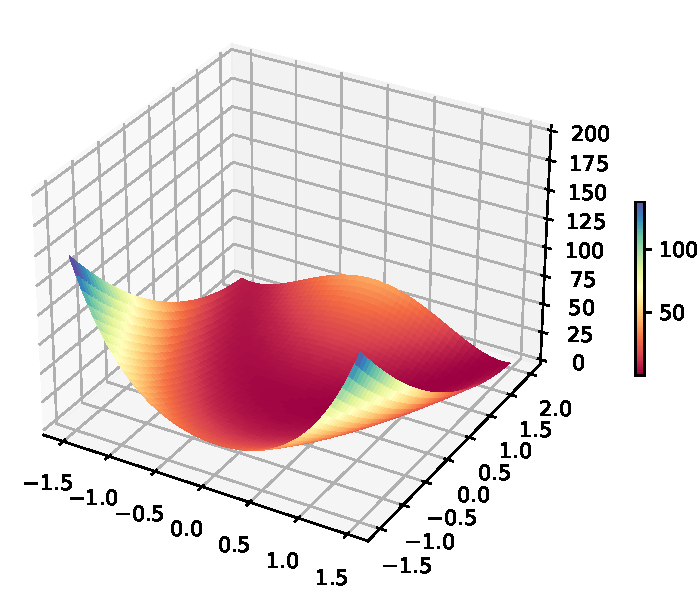
\includegraphics[width=0.40\linewidth]{img/rosenbrock.pdf}
		\caption{$f(x,y)=(a-x)^{2}+b(y-x^{2})^{2}, a = 1, b = 100$}
		%https://colab.research.google.com/drive/1mlZtxPXuk3mls56CQArmDzjdp5bLbrJC?usp=sharing
	\end{figure}
	$$\nabla f = \left(-400xy+400x^3+2x-2; \quad 200y-200x^2 \right)$$
	
\end{frame}

\begin{frame}{Gradient for minimizing multivariate functions}
	
	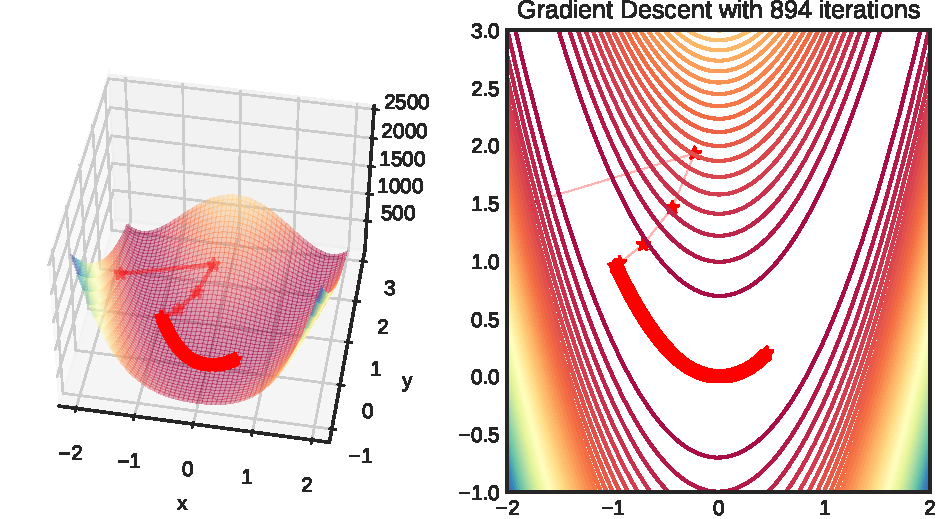
\includegraphics[width=0.86\linewidth]{img/gradient1.pdf}
	
	Random starting point $(-1.8; 1.5)$, minimum at $(1; 1)$ \\

{\tiny \url{https://colab.research.google.com/drive/1pTGjtbiQg3q08NGNkA7XgPMIQXf7uT76}}

	
\end{frame}

\section{Problem 3: When functions become heavily nested}


\begin{frame}{In reality we work with deeply composed functions}
	
	\begin{example}
		Minimize function $e$ wrt.\ $w_0, w_1, \ldots, w_K$
		$$
		e = - \frac{1}{N} \sum_{i = 1}^{N} y_{[i]} \log
		\left(
		\frac{1}{1 +
			\exp\left( w_0 + \sum_{j=1}^{K} w_k \cdot \bm{x}_{[i][k]} \right)
		}
		\right)
		$$
		Where $\bm{x}_{[1]}, \ldots, \bm{x}_{[N]},$ and $y_{[1]}, \ldots, y_{[N]}$ are constants
	\end{example}
	
	\pause
	
	$$
	\nabla f = \left( \pdv{e}{w_0}; \pdv{e}{w_1}; \ldots; \pdv{e}{w_K} \right)
	$$
	
	$\pdv{e}{w_1} = \ldots$ \pause Good luck!
	
\end{frame}


%\begin{frame}{Chain Rule for Multivariable Functions}
%	
%	
%	Suppose that $x=g(t)$ and $y=h(t)$ are differentiable functions of $t$ and $z=f(x,y)$ is a differentiable function of $x$ and $y$. Then $z=f(x(t),y(t))$ is a differentiable function of $t$ and
%	$$
%	\pdv{z}{t} =  \pdv{z}{x} \cdot \frac{dx}{dt} + \pdv{z}{y} \cdot \frac{dy}{dt}
%	$$
%	where the ordinary derivatives are evaluated at $t$ and the partial derivatives are evaluated at $(x,y)$.
%	
%	\pause
%	
%	\begin{block}{Be ready for possible notation madness}
%		$$
%		\pdv{f}{t} =  \pdv{f}{g} \pdv{g}{t} + \pdv{f}{h} \pdv{h}{t}
%		$$
%	\end{block}
%	
%\end{frame}


\begin{frame}{Chain rule for multivariable functions \\ (two independent variables)}
	
	Suppose $x=g(u,v)$ and $y=h(u,v)$ are differentiable functions of $u$ and $v$, and $z=f(x,y)$ is a differentiable function of $x$ and $y$. Then, $z=f(g(u,v),h(u,v))$ is a differentiable function of $u$ and $v$, and
	
	$$
	\frac{\partial z}{\partial u} = \frac{\partial z}{\partial x} \frac{\partial x}{\partial u} + \frac{\partial z}{\partial y} \frac{\partial y}{\partial u}
	$$
	$$
	\frac{\partial z}{\partial v} = \frac{\partial z}{\partial x} \frac{\partial x}{\partial v} + \frac{\partial z}{\partial y} \frac{\partial y}{\partial v}
	$$
	
\end{frame}

\subsection{Efficient computation of gradient}

\begin{frame}{Working example}
	
	$$
	e = (a + b)(b + 1)
	$$
	
	Compute gradient wrt.\ $a$ and $b$
	
	\bigskip
	
	\pause
	
	\begin{block}{This one is easy by hand, but that's not the point}
		$$
		e = (a + b)(b + 1) = ab + a + b^2 + b
		$$
		$$
		\pdv{e}{a} = b + 1 \qquad \pdv{e}{b} = a + 2b + 1
		$$
	\end{block}
	
\end{frame}



\begin{frame}{Add some intermediate variables and function names}
	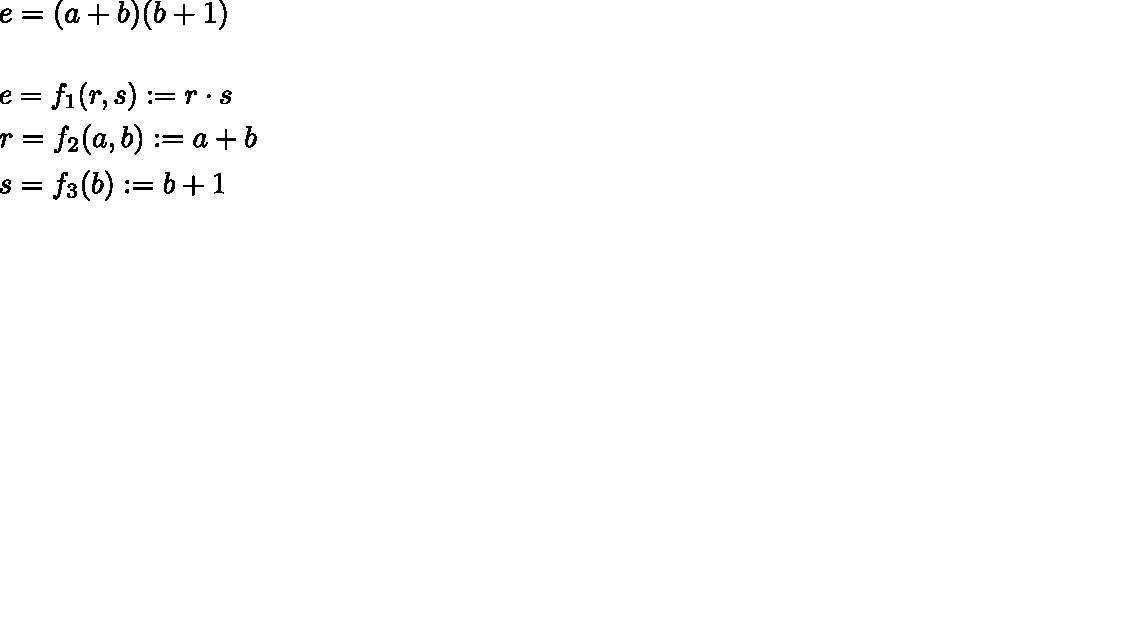
\includegraphics[width=1.1\linewidth]{img/backprop01.pdf}
\end{frame}

\begin{frame}{Build computational graph and evaluate (forward step)}
	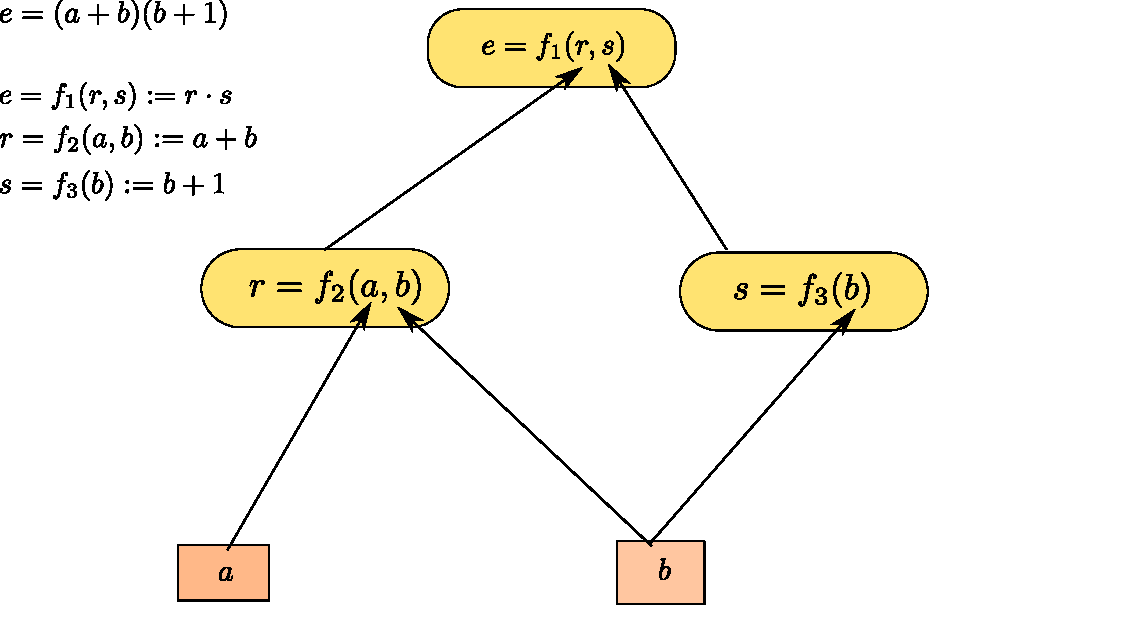
\includegraphics[width=1.1\linewidth]{img/backprop02.pdf}
	
	
	\begin{tikzpicture}[overlay, remember picture] 
		\node at (current page.north east)[anchor = north east, text width=4cm, yshift=-1.3cm] {\scriptsize \textbf{Important:} $a, b$ will be some concrete real numbers, therefore $r, s, e$ will be concrete real numbers too! \par};
	\end{tikzpicture}	
	
\end{frame}


\begin{frame}{Computational graph}
	\begin{itemize}
		\item DAG --- directed acyclic graph (not necessarily a tree!)
		\item Each node --- a differentiable function with arguments
		\item Leaves --- variables (e.g., $a, b$) or constants
		\item Arrows --- Function composition
	\end{itemize}
	
	\begin{figure}
		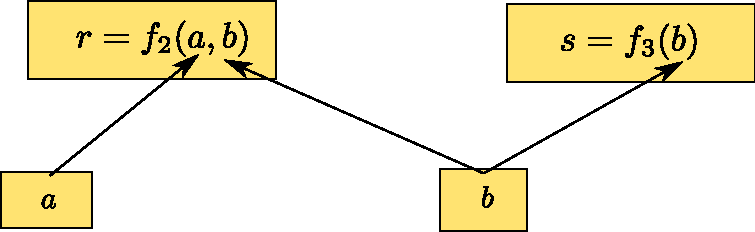
\includegraphics[width=0.75\linewidth]{img/parent-child.pdf}
		\caption{$r, s$ are parents of $b$; $a, b$ are children (arguments) of $r$}
	\end{figure}
	
	
	
\end{frame}

\begin{frame}{Goal: $\pdv{e}{a}$ and $\pdv{e}{b}$ (gradient), but let's do $\pdv{e}{\star}$ for every node}
	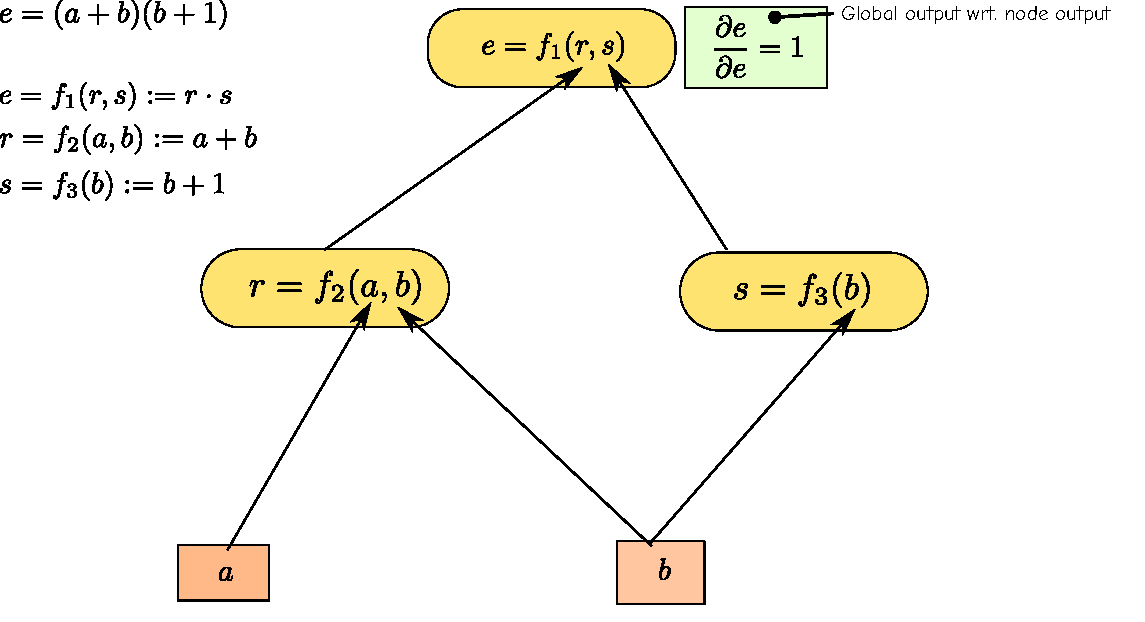
\includegraphics[width=1.1\linewidth]{img/backprop03.pdf}
\end{frame}

\begin{frame}{Since $e = r \cdot s$, partial derivatives are easy: $\pdv{e}{r} = s$ and $\pdv{e}{s} = r$}
	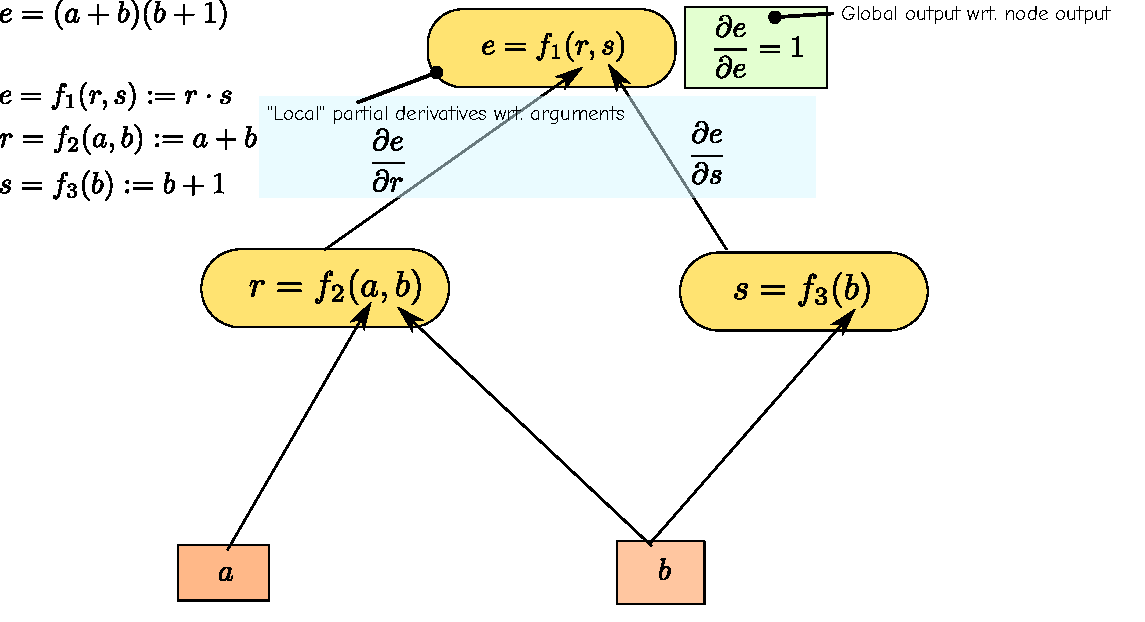
\includegraphics[width=1.1\linewidth]{img/backprop04.pdf}
	
	\begin{tikzpicture}[overlay, remember picture] 
		\node at (current page.north east)[anchor = north east, text width=4cm, yshift=-1.7cm] {\scriptsize \textbf{Sanity check:} $r, s$ are some concrete real numbers, therefore $\pdv{e}{r}$ and $\pdv{e}{s}$ will be concrete real numbers too! \par};
	\end{tikzpicture}
\end{frame}

\begin{frame}{Proceed to next child $r$ and compute $\pdv{e}{r}$ -- use chain rule!}
	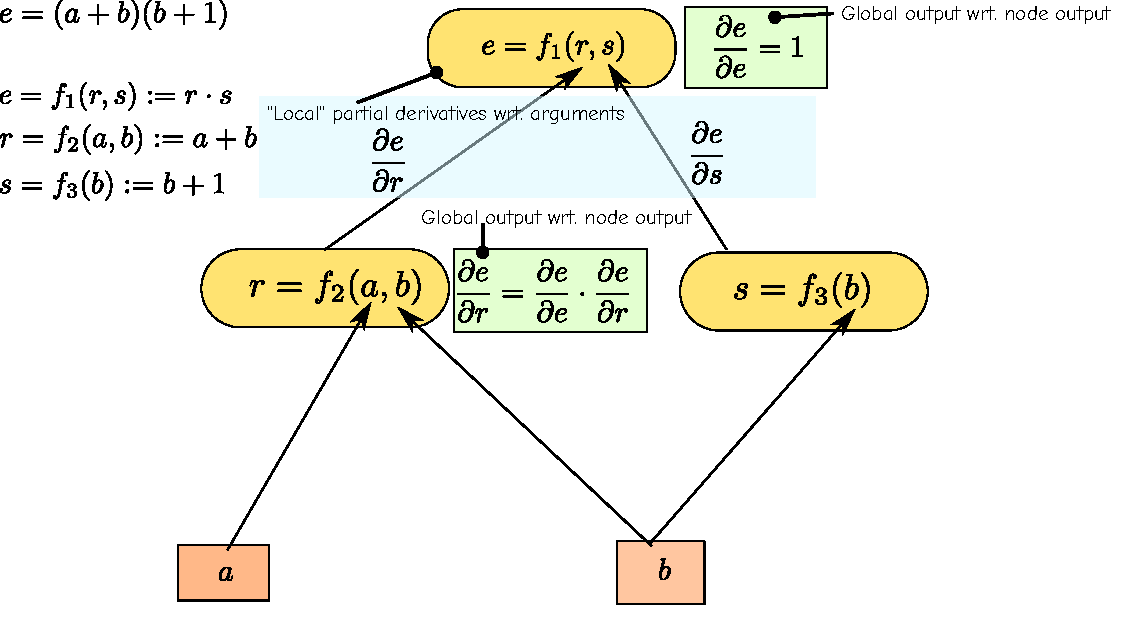
\includegraphics[width=1.1\linewidth]{img/backprop05.pdf}
	
	
\end{frame}

\begin{frame}{Proceed to next child $s$ and compute $\pdv{e}{s}$ -- use chain rule!}
	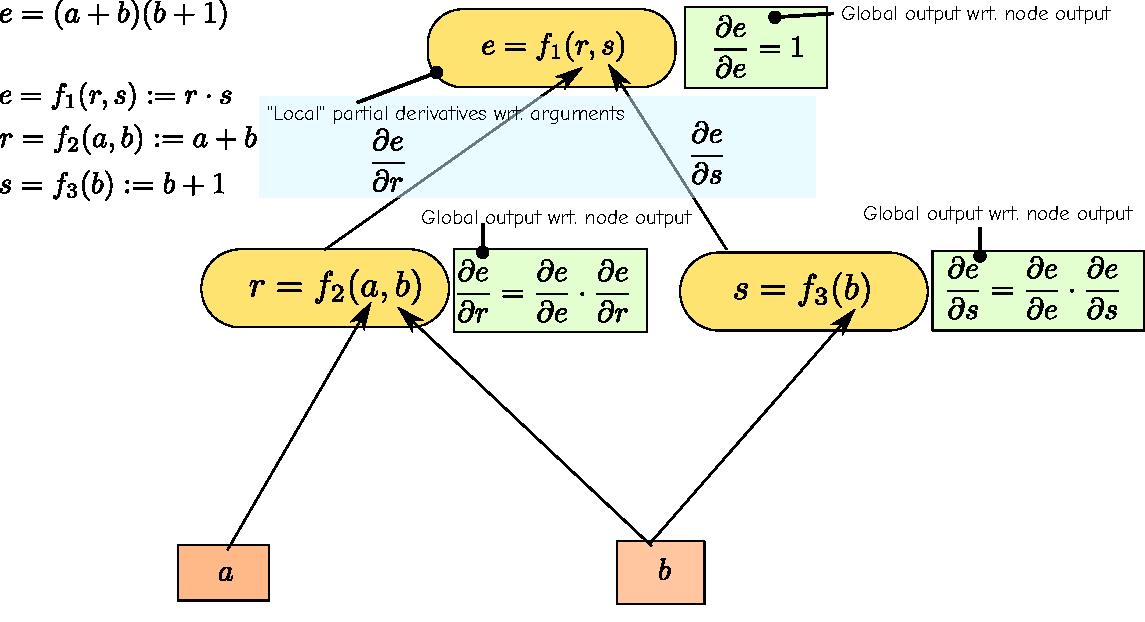
\includegraphics[width=1.1\linewidth]{img/backprop06.pdf}
\end{frame}

\begin{frame}{Since $r = a + b$, partial derivatives are easy: $\pdv{r}{a} = 1$ and $\pdv{r}{b} = 1$}
	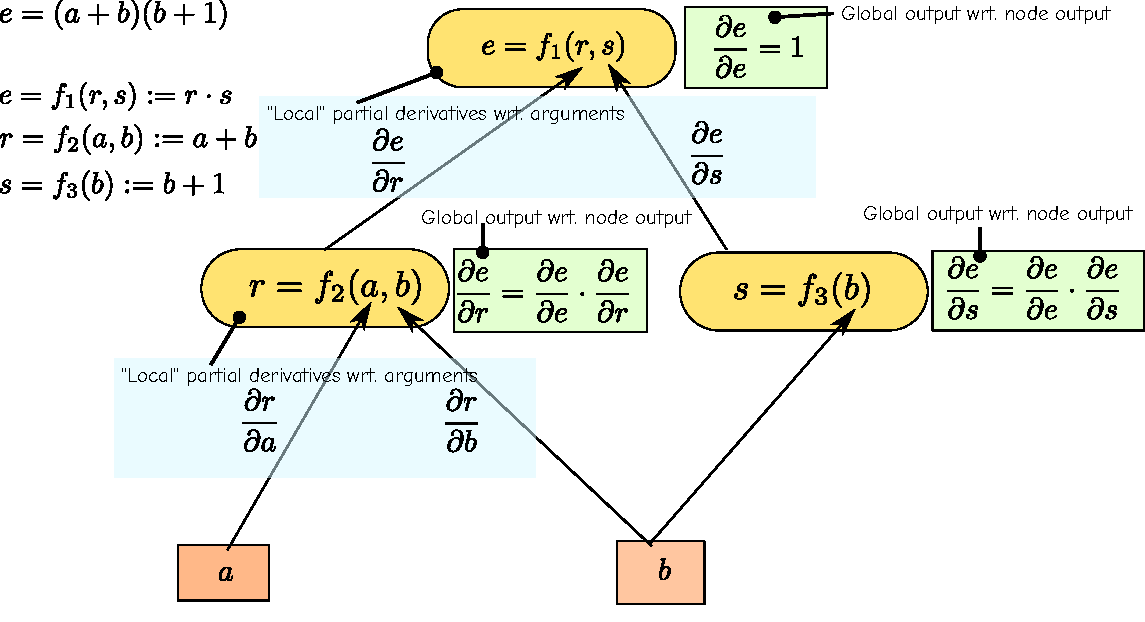
\includegraphics[width=1.1\linewidth]{img/backprop07.pdf}
\end{frame}

\begin{frame}{Proceed to next child $a$ and compute $\pdv{e}{a}$ -- use chain rule!}
	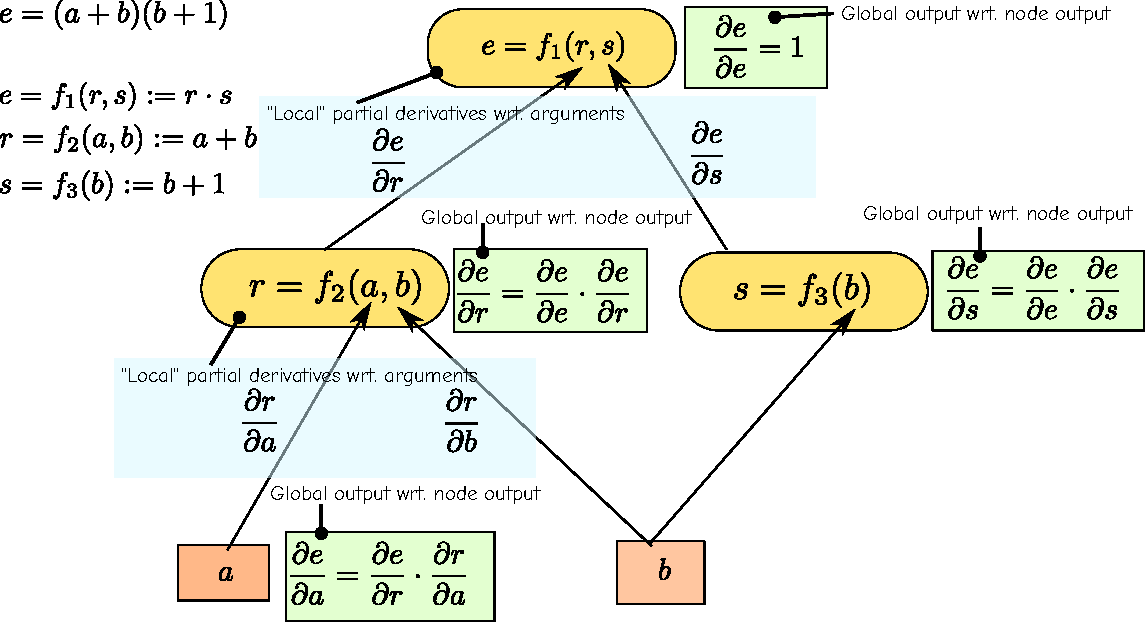
\includegraphics[width=1.1\linewidth]{img/backprop08.pdf}
\end{frame}

\begin{frame}{Since $s = b + 1$, partial derivatives are easy: $\pdv{s}{b} = 1$}
	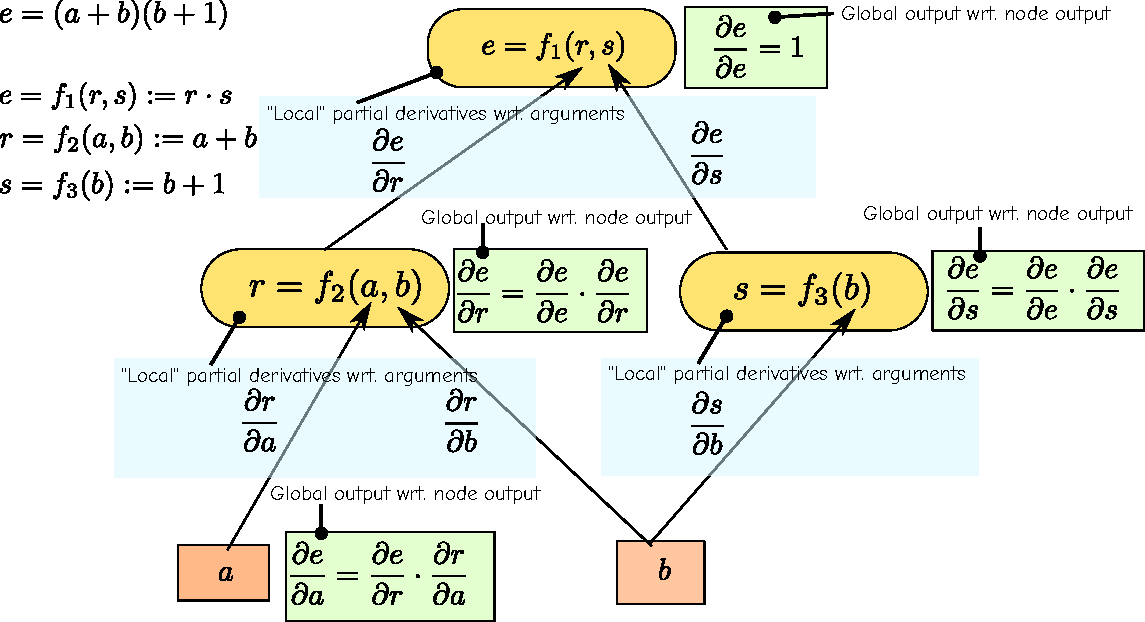
\includegraphics[width=1.1\linewidth]{img/backprop09.pdf}
\end{frame}

\begin{frame}{Proceed to $b$ and compute $\pdv{e}{b}$ -- use multivariate chain rule!}
	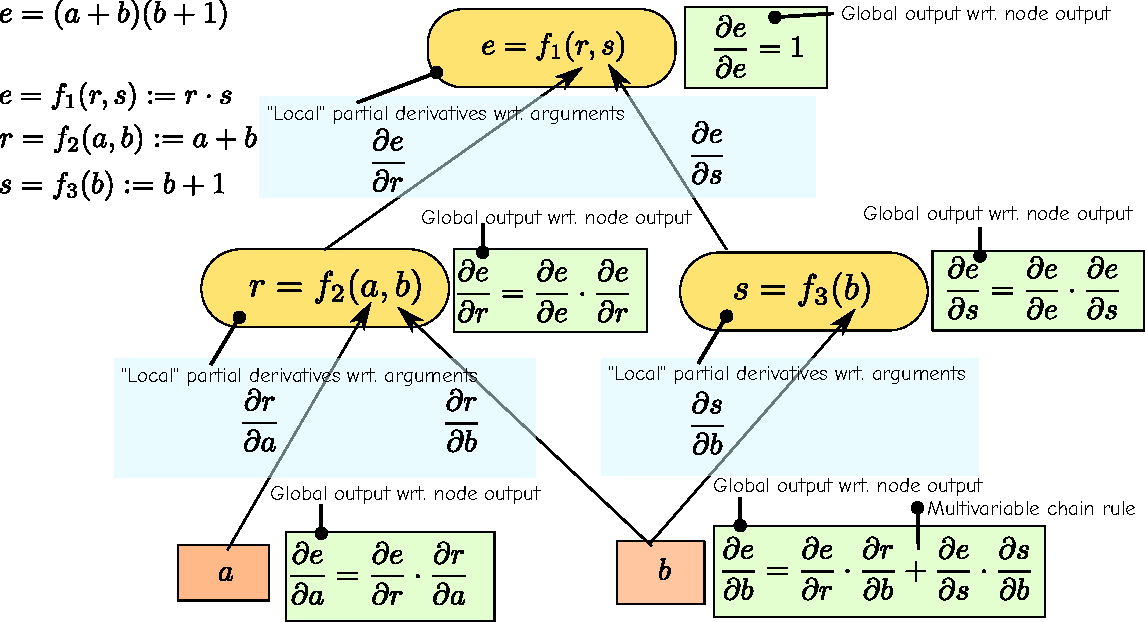
\includegraphics[width=1.1\linewidth]{img/backprop10.pdf}
\end{frame}


\begin{frame}{Goal: $\nabla e = \left( \pdv{e}{a}; \pdv{e}{b} \right)$ --- we computed it for concrete $a$ and $b$!}
	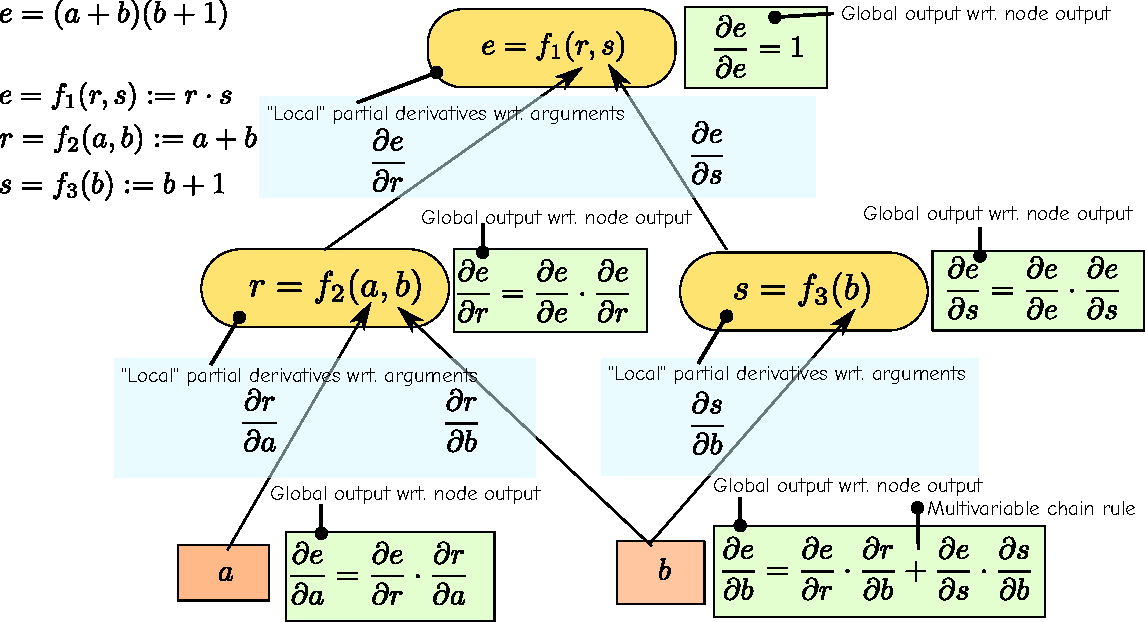
\includegraphics[width=1.1\linewidth]{img/backprop10.pdf}
\end{frame}


\begin{frame}{Generic node in a computational graph}
	
	
	
	
	
	
	\begin{figure}
		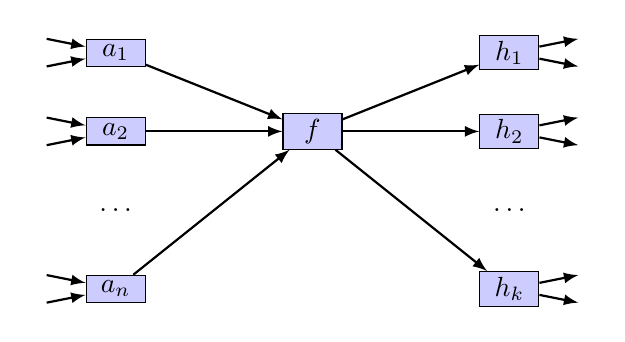
\begin{tikzpicture}	
			%\node (a1) [draw, circle, inner sep=0pt, minimum width=0.75cm, fill=green!20] {$a_1$};
			\node (a1) [neuron] {$a_1$};
			\node (a2) [neuron, below of=a1] {$a_2$};
			\node (dots1) [below of=a2] {$\ldots$};
			\node (an) [neuron, below of=dots1] {$a_n$};
			
			\node (f) [neuron, right of=a2, xshift=1.5cm] {$f$};
			
			\node (h2) [neuron, right of=f, xshift=1.5cm] {$h_2$};
			\node (h1) [neuron, above of=h2] {$h_1$};
			\node (dots2) [below of=h2] {$\ldots$};
			\node (hk) [neuron, below of=dots2] {$h_k$};
			
			% inputs
			\node (a1in1) [left of=a1, yshift=0.2cm] {};
			\node (a1in2) [left of=a1, yshift=-0.2cm] {};
			
			\node (a2in1) [left of=a2, yshift=0.2cm] {};
			\node (a2in2) [left of=a2, yshift=-0.2cm] {};
			
			\node (anin1) [left of=an, yshift=0.2cm] {};
			\node (anin2) [left of=an, yshift=-0.2cm] {};
			
			% outputs
			\node (h1o1) [right of=h1, yshift=0.2cm] {};
			\node (h1o2) [right of=h1, yshift=-0.2cm] {};
			
			\node (h2o1) [right of=h2, yshift=0.2cm] {};
			\node (h2o2) [right of=h2, yshift=-0.2cm] {};
			
			\node (hko1) [right of=hk, yshift=0.2cm] {};
			\node (hko2) [right of=hk, yshift=-0.2cm] {};
			
			
			\begin{scope}[thick, black, ->, >=latex]
				\draw (a1) -- (f);
				\draw (a2) -- (f);
				\draw (an) -- (f);
				\draw (f) -- (h1);
				\draw (f) -- (h2);
				\draw (f) -- (hk);
				
				\draw (a1in1) -- (a1);
				\draw (a1in2) -- (a1);
				\draw (a2in1) -- (a2);
				\draw (a2in2) -- (a2);
				\draw (anin1) -- (an);
				\draw (anin2) -- (an);
				
				\draw (h1) -- (h1o1);
				\draw (h1) -- (h1o2);
				\draw (h2) -- (h2o1);
				\draw (h2) -- (h2o2);
				\draw (hk) -- (hko1);
				\draw (hk) -- (hko2);
			\end{scope}	
		\end{tikzpicture}
		
		
		\caption{A generic node of a computation graph. Node $f$ has many inputs, its output
			feeds into many nodes, and each of its inputs and outputs may also have many inputs
			and outputs.}
	\end{figure}
	

	\begin{tikzpicture}[overlay, remember picture] 
		\node at (current page.north east)[ref] {Adapted from \fullcite[p.~265]{Kun.2020} \par};
	\end{tikzpicture}
	
\end{frame}


\begin{frame}{Generic node in a computational graph $f(a_1, \ldots, a_n)$}
	
	\begin{figure}
		\scalebox{0.6}{%
			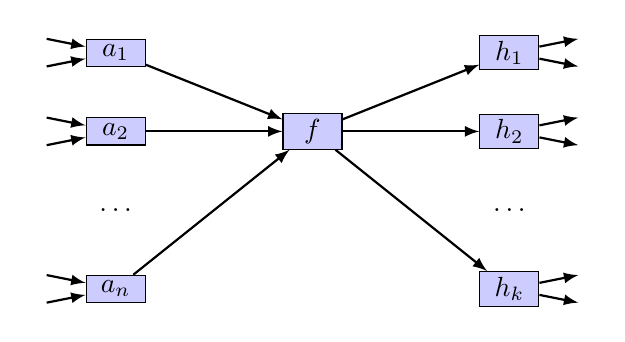
\begin{tikzpicture}
				%\node (a1) [draw, circle, inner sep=0pt, minimum width=0.75cm, fill=green!20] {$a_1$};
				\node (a1) [neuron] {$a_1$};
				\node (a2) [neuron, below of=a1] {$a_2$};
				\node (dots1) [below of=a2] {$\ldots$};
				\node (an) [neuron, below of=dots1] {$a_n$};
				
				\node (f) [neuron, right of=a2, xshift=1.5cm] {$f$};
				
				\node (h2) [neuron, right of=f, xshift=1.5cm] {$h_2$};
				\node (h1) [neuron, above of=h2] {$h_1$};
				\node (dots2) [below of=h2] {$\ldots$};
				\node (hk) [neuron, below of=dots2] {$h_k$};
				
				% inputs
				\node (a1in1) [left of=a1, yshift=0.2cm] {};
				\node (a1in2) [left of=a1, yshift=-0.2cm] {};
				
				\node (a2in1) [left of=a2, yshift=0.2cm] {};
				\node (a2in2) [left of=a2, yshift=-0.2cm] {};
				
				\node (anin1) [left of=an, yshift=0.2cm] {};
				\node (anin2) [left of=an, yshift=-0.2cm] {};
				
				% outputs
				\node (h1o1) [right of=h1, yshift=0.2cm] {};
				\node (h1o2) [right of=h1, yshift=-0.2cm] {};
				
				\node (h2o1) [right of=h2, yshift=0.2cm] {};
				\node (h2o2) [right of=h2, yshift=-0.2cm] {};
				
				\node (hko1) [right of=hk, yshift=0.2cm] {};
				\node (hko2) [right of=hk, yshift=-0.2cm] {};
				
				
				\begin{scope}[thick, black, ->, >=latex]
					\draw (a1) -- (f);
					\draw (a2) -- (f);
					\draw (an) -- (f);
					\draw (f) -- (h1);
					\draw (f) -- (h2);
					\draw (f) -- (hk);
					
					\draw (a1in1) -- (a1);
					\draw (a1in2) -- (a1);
					\draw (a2in1) -- (a2);
					\draw (a2in2) -- (a2);
					\draw (anin1) -- (an);
					\draw (anin2) -- (an);
					
					\draw (h1) -- (h1o1);
					\draw (h1) -- (h1o2);
					\draw (h2) -- (h2o1);
					\draw (h2) -- (h2o2);
					\draw (hk) -- (hko1);
					\draw (hk) -- (hko2);
				\end{scope}	
			\end{tikzpicture}
		}
	\end{figure}
	
	
	Assuming the graph is a function $e = g(\ldots)$, we compute
	$$\pdv{e}{f} = \sum_{i = 1}^{k} \pdv{e}{h_i} \cdot \pdv{h_i}{f}$$
	and
	$$\pdv{f}{a_i} \quad \text{for } a_i, \ldots, a_n$$
	
\end{frame}

\begin{frame}{What each node must implement?}
	
	For example a function $s = f(a, b, c, d)$
	
	\begin{itemize}
		\item How to compute the output value $s$ (given the parameters $a, b, c, d$)
		\item How to compute partial derivatives wrt.\ the parameters, i.e. $\pdv{s}{a}, \pdv{s}{b}, \pdv{s}{c}, \pdv{s}{d}$
	\end{itemize}
	
\end{frame}

\begin{frame}{Backpropagation}
	
	\begin{itemize}
		\item Forward computation: Compute all nodes' output (and cache it)
		\item Backward computation (Backprop): Compute the overall function's partial derivative with respect to each node
	\end{itemize}
	
	\bigskip
	
	Ordering of the computations? Recursively or build a graph's topology upfront and iterate
	
\end{frame}


\begin{frame}{Backpropagation: Recap}
	\begin{itemize}
		\item We can express any arbitrarily complicated function $f: \mathbb{R}^n \to \mathbb{R}$ as a computational graph
		\item For computing the gradient $\nabla f$ at a concrete point $(x_1, x_2, \ldots, x_n)$ we run the forward pass and backprop
		\item When caching each node's intermediate output and partial derivatives, we avoid repeating computations $\to$ efficient algorithm
	\end{itemize}
\end{frame}


\section*{Recap}

\begin{frame}{Take aways}
	
	\begin{itemize}
		
		\item We can quite efficiently find a minimum of any differentiable nested multivariate function
		\begin{itemize}
			\item Iterative gradient descent takes the most promising direction
			\item Backpropagation utilizes computational graphs and caching $\to$ computes gradients efficiently
		\end{itemize}
		\item We have not touched neural networks yet at all!
	\end{itemize}
	
\end{frame}



\begin{frame}{License and credits}
	
	\begin{columns}
		\begin{column}{0.7\textwidth}
			Licensed under Creative Commons Attribution-ShareAlike 4.0 International (CC BY-SA 4.0)
		\end{column}
		\begin{column}{0.2\textwidth}
			
\includegraphics[width=0.9\linewidth]{img/cc-by-sa-icon.pdf}
		\end{column}
	\end{columns}
	
	\bigskip
	
	Credits
	
	\begin{scriptsize}
		
		Ivan Habernal
		
		Content from ACL Anthology papers licensed under CC-BY \url{https://www.aclweb.org/anthology}
		
	\end{scriptsize}
	
\end{frame}


\end{document}

